% Options for packages loaded elsewhere
\PassOptionsToPackage{unicode}{hyperref}
\PassOptionsToPackage{hyphens}{url}
%
\documentclass[
]{book}
\usepackage{amsmath,amssymb}
\usepackage{lmodern}
\usepackage{iftex}
\ifPDFTeX
  \usepackage[T1]{fontenc}
  \usepackage[utf8]{inputenc}
  \usepackage{textcomp} % provide euro and other symbols
\else % if luatex or xetex
  \usepackage{unicode-math}
  \defaultfontfeatures{Scale=MatchLowercase}
  \defaultfontfeatures[\rmfamily]{Ligatures=TeX,Scale=1}
\fi
% Use upquote if available, for straight quotes in verbatim environments
\IfFileExists{upquote.sty}{\usepackage{upquote}}{}
\IfFileExists{microtype.sty}{% use microtype if available
  \usepackage[]{microtype}
  \UseMicrotypeSet[protrusion]{basicmath} % disable protrusion for tt fonts
}{}
\makeatletter
\@ifundefined{KOMAClassName}{% if non-KOMA class
  \IfFileExists{parskip.sty}{%
    \usepackage{parskip}
  }{% else
    \setlength{\parindent}{0pt}
    \setlength{\parskip}{6pt plus 2pt minus 1pt}}
}{% if KOMA class
  \KOMAoptions{parskip=half}}
\makeatother
\usepackage{xcolor}
\IfFileExists{xurl.sty}{\usepackage{xurl}}{} % add URL line breaks if available
\IfFileExists{bookmark.sty}{\usepackage{bookmark}}{\usepackage{hyperref}}
\hypersetup{
  pdftitle={CSAFE Computing Resources},
  pdfauthor={Stephanie Reinders},
  hidelinks,
  pdfcreator={LaTeX via pandoc}}
\urlstyle{same} % disable monospaced font for URLs
\usepackage{color}
\usepackage{fancyvrb}
\newcommand{\VerbBar}{|}
\newcommand{\VERB}{\Verb[commandchars=\\\{\}]}
\DefineVerbatimEnvironment{Highlighting}{Verbatim}{commandchars=\\\{\}}
% Add ',fontsize=\small' for more characters per line
\usepackage{framed}
\definecolor{shadecolor}{RGB}{248,248,248}
\newenvironment{Shaded}{\begin{snugshade}}{\end{snugshade}}
\newcommand{\AlertTok}[1]{\textcolor[rgb]{0.94,0.16,0.16}{#1}}
\newcommand{\AnnotationTok}[1]{\textcolor[rgb]{0.56,0.35,0.01}{\textbf{\textit{#1}}}}
\newcommand{\AttributeTok}[1]{\textcolor[rgb]{0.77,0.63,0.00}{#1}}
\newcommand{\BaseNTok}[1]{\textcolor[rgb]{0.00,0.00,0.81}{#1}}
\newcommand{\BuiltInTok}[1]{#1}
\newcommand{\CharTok}[1]{\textcolor[rgb]{0.31,0.60,0.02}{#1}}
\newcommand{\CommentTok}[1]{\textcolor[rgb]{0.56,0.35,0.01}{\textit{#1}}}
\newcommand{\CommentVarTok}[1]{\textcolor[rgb]{0.56,0.35,0.01}{\textbf{\textit{#1}}}}
\newcommand{\ConstantTok}[1]{\textcolor[rgb]{0.00,0.00,0.00}{#1}}
\newcommand{\ControlFlowTok}[1]{\textcolor[rgb]{0.13,0.29,0.53}{\textbf{#1}}}
\newcommand{\DataTypeTok}[1]{\textcolor[rgb]{0.13,0.29,0.53}{#1}}
\newcommand{\DecValTok}[1]{\textcolor[rgb]{0.00,0.00,0.81}{#1}}
\newcommand{\DocumentationTok}[1]{\textcolor[rgb]{0.56,0.35,0.01}{\textbf{\textit{#1}}}}
\newcommand{\ErrorTok}[1]{\textcolor[rgb]{0.64,0.00,0.00}{\textbf{#1}}}
\newcommand{\ExtensionTok}[1]{#1}
\newcommand{\FloatTok}[1]{\textcolor[rgb]{0.00,0.00,0.81}{#1}}
\newcommand{\FunctionTok}[1]{\textcolor[rgb]{0.00,0.00,0.00}{#1}}
\newcommand{\ImportTok}[1]{#1}
\newcommand{\InformationTok}[1]{\textcolor[rgb]{0.56,0.35,0.01}{\textbf{\textit{#1}}}}
\newcommand{\KeywordTok}[1]{\textcolor[rgb]{0.13,0.29,0.53}{\textbf{#1}}}
\newcommand{\NormalTok}[1]{#1}
\newcommand{\OperatorTok}[1]{\textcolor[rgb]{0.81,0.36,0.00}{\textbf{#1}}}
\newcommand{\OtherTok}[1]{\textcolor[rgb]{0.56,0.35,0.01}{#1}}
\newcommand{\PreprocessorTok}[1]{\textcolor[rgb]{0.56,0.35,0.01}{\textit{#1}}}
\newcommand{\RegionMarkerTok}[1]{#1}
\newcommand{\SpecialCharTok}[1]{\textcolor[rgb]{0.00,0.00,0.00}{#1}}
\newcommand{\SpecialStringTok}[1]{\textcolor[rgb]{0.31,0.60,0.02}{#1}}
\newcommand{\StringTok}[1]{\textcolor[rgb]{0.31,0.60,0.02}{#1}}
\newcommand{\VariableTok}[1]{\textcolor[rgb]{0.00,0.00,0.00}{#1}}
\newcommand{\VerbatimStringTok}[1]{\textcolor[rgb]{0.31,0.60,0.02}{#1}}
\newcommand{\WarningTok}[1]{\textcolor[rgb]{0.56,0.35,0.01}{\textbf{\textit{#1}}}}
\usepackage{longtable,booktabs,array}
\usepackage{calc} % for calculating minipage widths
% Correct order of tables after \paragraph or \subparagraph
\usepackage{etoolbox}
\makeatletter
\patchcmd\longtable{\par}{\if@noskipsec\mbox{}\fi\par}{}{}
\makeatother
% Allow footnotes in longtable head/foot
\IfFileExists{footnotehyper.sty}{\usepackage{footnotehyper}}{\usepackage{footnote}}
\makesavenoteenv{longtable}
\usepackage{graphicx}
\makeatletter
\def\maxwidth{\ifdim\Gin@nat@width>\linewidth\linewidth\else\Gin@nat@width\fi}
\def\maxheight{\ifdim\Gin@nat@height>\textheight\textheight\else\Gin@nat@height\fi}
\makeatother
% Scale images if necessary, so that they will not overflow the page
% margins by default, and it is still possible to overwrite the defaults
% using explicit options in \includegraphics[width, height, ...]{}
\setkeys{Gin}{width=\maxwidth,height=\maxheight,keepaspectratio}
% Set default figure placement to htbp
\makeatletter
\def\fps@figure{htbp}
\makeatother
\setlength{\emergencystretch}{3em} % prevent overfull lines
\providecommand{\tightlist}{%
  \setlength{\itemsep}{0pt}\setlength{\parskip}{0pt}}
\setcounter{secnumdepth}{5}
\usepackage{booktabs}
\ifLuaTeX
  \usepackage{selnolig}  % disable illegal ligatures
\fi
\usepackage[]{natbib}
\bibliographystyle{plainnat}

\title{CSAFE Computing Resources}
\author{Stephanie Reinders}
\date{2022-06-10}

\begin{document}
\maketitle

{
\setcounter{tocdepth}{1}
\tableofcontents
}
\hypertarget{introduction}{%
\chapter{Introduction}\label{introduction}}

This book gives the reader step-by-step instructions for accessing and using several CSAFE computing resources. CSAFE has access to

\begin{enumerate}
\def\labelenumi{\arabic{enumi}.}
\tightlist
\item
  Large Scale Storage (LSS)
\item
  CSAFE Rstudio Servers
\item
  The Pronto Job Scheduler
\end{enumerate}

\hypertarget{large-scale-storage-lss}{%
\section{Large Scale Storage (LSS)}\label{large-scale-storage-lss}}

ResearchIT at Iowa State University provides Large Scale Storage (LSS) at low cost to research labs. CSAFE has purchased more than 30 terabytes of space on LSS. As of 2022-06-10 the following CSAFE project folders are on LSS:

\begin{itemize}
\tightlist
\item
  csafe-admin-vid
\item
  csafe-firearms
\item
  csafe-handwriting
\item
  csafe-handwriting-irb
\item
  csafe-mentisdb
\item
  csafe-mobile
\item
  csafe-shoeprints
\item
  csafe-stego
\item
  csafe-transcripts
\item
  csafe-wvmediaimp
\end{itemize}

Chapter \ref{lss} explains how to connect to LSS.

\hypertarget{csafe-rstudio-servers}{%
\section{CSAFE RStudio Servers}\label{csafe-rstudio-servers}}

CSAFE has access to two RStudio Servers. To the user, the experience is almost exactly the same as using RStudio on a personal computer. The main benefit of running RStudio on the server is that the server has more RAM and more cores than most personal computers.

Chapter \ref{rstudio-server} explains how to use the Rstudio servers.

\hypertarget{the-pronto-job-scheduler}{%
\section{The Pronto Job Scheduler}\label{the-pronto-job-scheduler}}

ResearchIT at ISU manages a whole host of high performance servers to which CSAFE has purchased access. Instead of accessing one of these servers individually, users submit their jobs (scripts) to the Pronto Job Scheduler which assigns the jobs to the most appropriate servers.

Chapter \ref{pronto} explains how to run R scripts on the Pronto Job Scheduler. Python, MATLAB, and other programming languages can be run on Pronto, but this book only covers R.

\hypertarget{do-i-use-the-csafe-rstudio-server-or-pronto}{%
\section{Do I use the CSAFE Rstudio Server or Pronto?}\label{do-i-use-the-csafe-rstudio-server-or-pronto}}

When deciding whether to use an RStudio server or Pronto, you might want to consider the following benefits and drawbacks of each.

\textbf{RStudio Server}

\begin{itemize}
\tightlist
\item
  \emph{benefits}

  \begin{itemize}
  \tightlist
  \item
    It runs the RStudio graphical user interface so the user experience is quite similar to working in Rstudio on a personal computer.
  \end{itemize}
\item
  \emph{drawbacks}

  \begin{itemize}
  \tightlist
  \item
    Each server has less than 20 cores
  \item
    It is a shared user machine which means that if a lot of people are using the server, your jobs might run slower.
  \end{itemize}
\end{itemize}

\textbf{Pronto}

\begin{itemize}
\tightlist
\item
  \emph{benefits}

  \begin{itemize}
  \tightlist
  \item
    It has dozens of servers with hundreds of cores each
  \item
    It manages the resources for users so you don't have to worry about slowing down other peoples jobs
  \end{itemize}
\item
  \emph{drawbacks}

  \begin{itemize}
  \tightlist
  \item
    It doesn't have a graphical user interface so users interact with Pronto through the command line
  \item
    Users submit their jobs to Pronto using something called a SLURM script, which is quite a different workflow compared running scripts in Rstudio
  \end{itemize}
\end{itemize}

\hypertarget{getting-started}{%
\chapter{Getting Started}\label{getting-started}}

If you are working from off campus you need to use ISU's virtual private network (VPN) to connect to any of the computing resources covered in this guide. You also need to set up SSH keys. Section \ref@(off-campus) explains how to install and use the ISU VPN and SSH keys. If you will only be working on campus, you may skip this section.

This chapter also includes a Quick Start Guide (Section \ref@(quick-start)) for people who are already comfortable with virtual private networks and command line prompts.

The last section in this chapter explains how people are granted access to the computing resources covered in this guide.

\hypertarget{quick-start}{%
\section{Quick Start Guide}\label{quick-start}}

\hypertarget{connect-to-large-scale-storage}{%
\subsection{Connect to Large Scale Storage}\label{connect-to-large-scale-storage}}

\begin{enumerate}
\def\labelenumi{\arabic{enumi}.}
\tightlist
\item
  If you are an undergraduate student, use your CSAFE email net-id and password in the following steps.
\item
  If you are off campus, download the ISU virtual private from \url{https://vpn.iastate.edu} and log-in using your ISU net-id and password.
\item
  On \textbf{Windows} open File Explorer and in the top textbox type

  \begin{itemize}
  \tightlist
  \item
    \texttt{\textbackslash{}\textbackslash{}las.iastate.edu\textbackslash{}research} if you are \textbf{on campus} or
  \item
    \texttt{\textbackslash{}\textbackslash{}las-dfs-01.las.iastate.edu\textbackslash{}lss} if you are \textbf{off campus}.
  \end{itemize}
\item
  On \textbf{Mac} click Go \textgreater{} Connect to Server and type

  \begin{itemize}
  \tightlist
  \item
    \texttt{smb://iastate/lss/research} if you are \textbf{on campus} or
  \item
    \texttt{smb://las-dfs-01.las.iastate.edu} if you are \textbf{off campus}.
  \end{itemize}
\item
  Enter your net-id and password.
\item
  Open the research folder and go to your CSAFE project folder.
\end{enumerate}

\hypertarget{connect-to-csafe-rstudio-server}{%
\subsection{Connect to CSAFE Rstudio Server}\label{connect-to-csafe-rstudio-server}}

\begin{enumerate}
\def\labelenumi{\arabic{enumi}.}
\tightlist
\item
  If you are an undergraduate student, use your CSAFE email net-id and password in the following steps.
\item
  If you are off campus, download the ISU virtual private from \url{https://vpn.iastate.edu} and log-in using your ISU net-id and password.
\item
  Go to the website \url{https://reiss.csafe.iastate.edu/} or \url{https://locard.csafe.iastate.edu/}.
\item
  Enter your net-id and password.
\end{enumerate}

\hypertarget{connect-to-the-pronto-job-scheduler}{%
\subsection{Connect to the Pronto Job Scheduler}\label{connect-to-the-pronto-job-scheduler}}

\begin{enumerate}
\def\labelenumi{\arabic{enumi}.}
\tightlist
\item
  If you are an undergraduate student, use your CSAFE email net-id and password in the following steps.
\item
  If you are off campus, download the ISU virtual private from \url{https://vpn.iastate.edu} and log-in using your ISU net-id and password.
\item
  On \textbf{Windows} open the PowerShell. On \textbf{Mac} open the Terminal.
\item
  Type \texttt{ssh\ your-netid@pronto.las.iastate.edu}
\item
  Enter your net-id and password.
\end{enumerate}

\hypertarget{off-campus}{%
\section{Working Off Campus}\label{off-campus}}

If you are on campus, you may skip this section. If you are off campus, you will need to

\begin{enumerate}
\def\labelenumi{\arabic{enumi}.}
\tightlist
\item
  Download and sign in to a virtual private network (see \ref{install-vpn})
\item
  Generate SSH keys (see \ref{ssh-keys})
\end{enumerate}

\hypertarget{install-vpn}{%
\subsection{Install the ISU Virtual Private Network (VPN)}\label{install-vpn}}

Iowa State University uses Cisco AnyConnect as their virtual private network (VPN) software. You will need to install it on your computer.

\begin{enumerate}
\def\labelenumi{\arabic{enumi}.}
\item
  Go to \url{https://vpn.iastate.edu}
\item
  Select Primary as the GROUP and click Login

  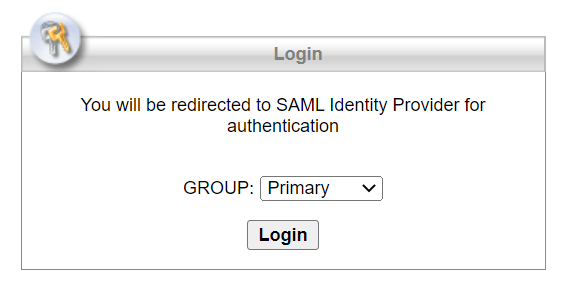
\includegraphics[width=0.5\textwidth,height=0.5\textheight]{images/group_primary.png}
\item
  Sign in with your ISU net-id and password

  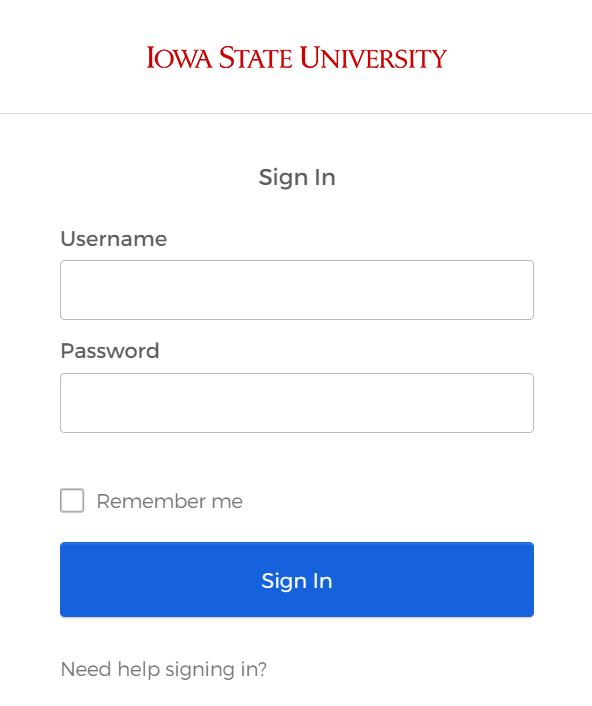
\includegraphics[width=0.3\textwidth,height=0.3\textheight]{images/isu_login.png}
\item
  The site should detect your computer's operating system and give you the option to download the VPN for your operating system.

  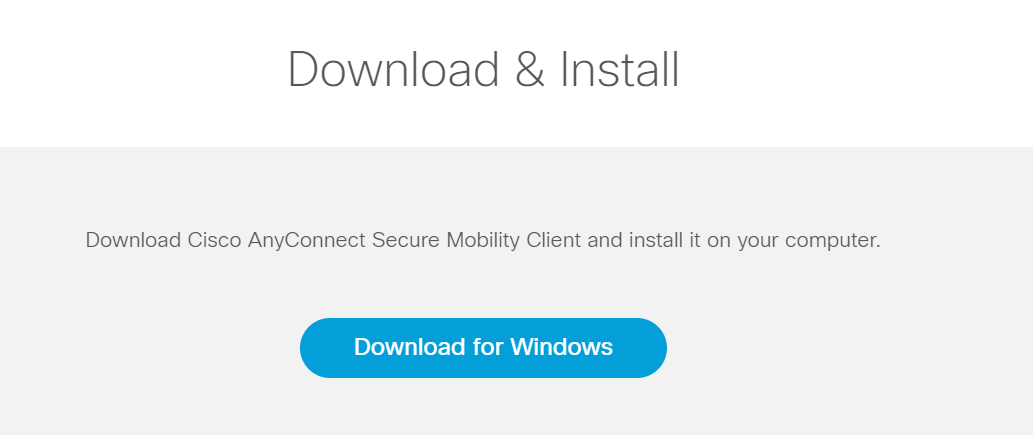
\includegraphics[width=0.5\textwidth,height=0.5\textheight]{images/cisco_detect_os.png}
\item
  Click Download
  \#\#\# Sign In to the ISU VPN \{\#signin-vpn\}
\item
  Open Cisco AnyConnect
\item
  Type \texttt{vpn.iastate.edu} and click Connect

  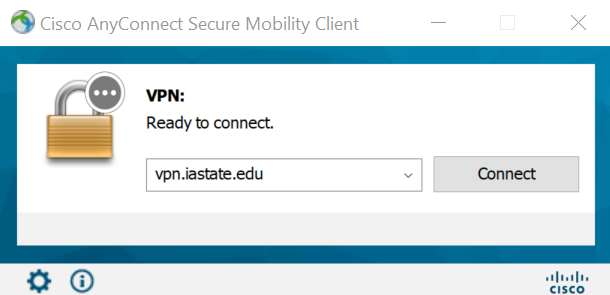
\includegraphics[width=0.5\textwidth,height=0.5\textheight]{images/cisco.png}
\item
  Sign in with your ISU net-id and password

  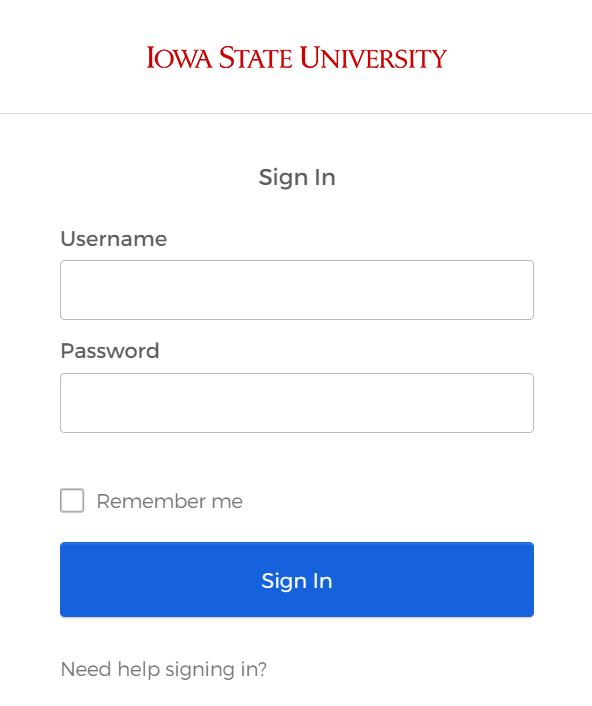
\includegraphics[width=0.3\textwidth,height=0.3\textheight]{images/isu_login.png}
\end{enumerate}

\hypertarget{ssh-keys}{%
\subsection{Generate SSH keys}\label{ssh-keys}}

ResearchIT gives instructions for setting up SSH keys at \url{https://researchit.las.iastate.edu/how-generate-ssh-keys}. Setting up my SSH keys took lots of trial and error. If you run into problems or get stuck, email \href{mailto:researchit@iastate.edu}{\nolinkurl{researchit@iastate.edu}}.

\hypertarget{lss}{%
\chapter{Large Scale Storage (LSS)}\label{lss}}

The Large Scale Storage (LSS) is a research file storage service at ISU. CSAFE has purchased storage space on LSS for a handful of CSAFE projects, such as firearms and handwriting, to store project data.

*** Add discussion of folder privileges and their impact on storing IRB data on the server

\textbf{Windows}

\begin{enumerate}
\def\labelenumi{\arabic{enumi}.}
\tightlist
\item
  If you are \textbf{off campus}, log-in to the ISU VPN
\item
  Open file explorer
\item
  If you are \textbf{off campus} type \texttt{\textbackslash{}\textbackslash{}las-dfs-01.las.iastate.edu\textbackslash{}lss} in the top textbox. If you are \textbf{on campus} you only need to type \texttt{\textbackslash{}\textbackslash{}las.iastate.edu\textbackslash{}lss}
\item
  Enter your ISU net-id and password
\item
  Open the research folder
\item
  Open folder for your CSAFE project
\end{enumerate}

\textbf{Mac}

\begin{enumerate}
\def\labelenumi{\arabic{enumi}.}
\tightlist
\item
  If you are off campus, log-in to the ISU VPN
\item
  Select Go \textgreater{} Connect to Server

  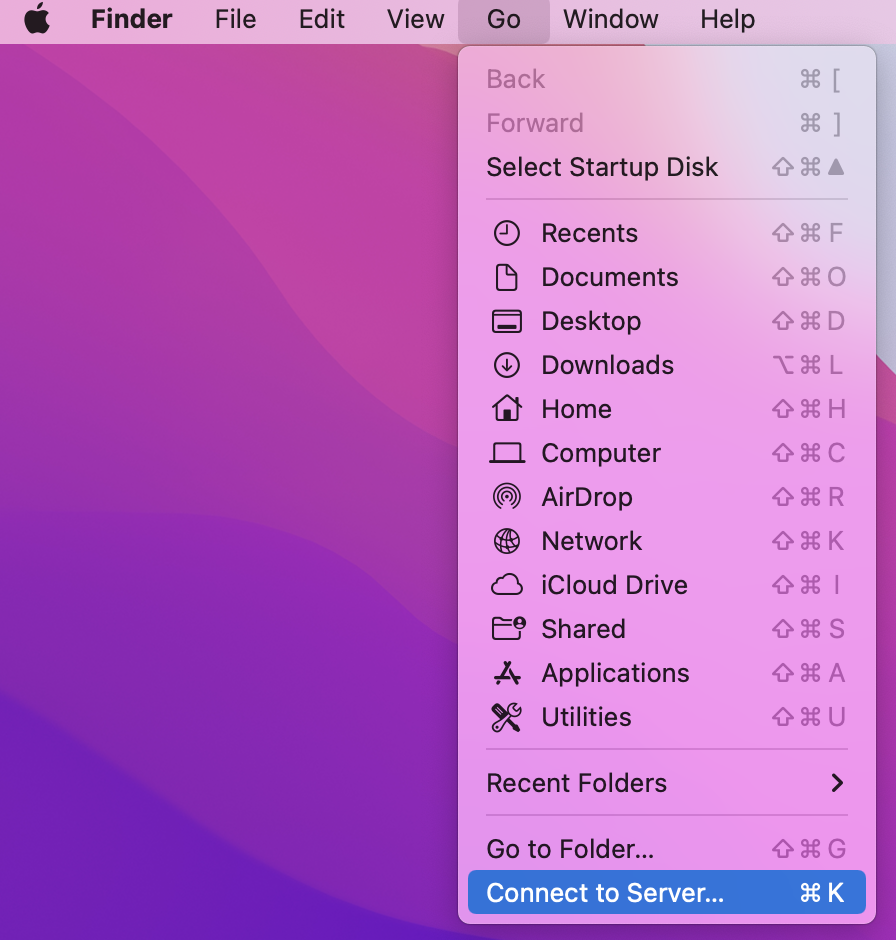
\includegraphics[width=0.5\textwidth,height=0.5\textheight]{images/connect_to_server.png}
\item
  If you are \textbf{off campus} type \texttt{smb://las-dfs-01.las.iastate.edu} in the text box. If you are \textbf{on campus} type \texttt{smb://las.iastate.edu} Click the + sign if you would like your computer to remember the server
\item
  Click Connect
\item
  Enter your net-id and password
\item
  Open the LSS folder
\item
  Open the research folder
\item
  Open folder for your CSAFE project
\end{enumerate}

\hypertarget{rstudio-server}{%
\chapter{The CSAFE RStudio Servers}\label{rstudio-server}}

CSAFE has two RStudio Servers that are operated by CSSM:

\begin{enumerate}
\def\labelenumi{\arabic{enumi}.}
\tightlist
\item
  \url{https://reiss.csafe.iastate.edu/}
\item
  \url{https://locard.csafe.iastate.edu/}
\end{enumerate}

*** Email \href{mailto:cssm_it@iastate.edu}{\nolinkurl{cssm\_it@iastate.edu}} for help

\hypertarget{connect-to-an-rstudio-server}{%
\section{Connect to an RStudio Server}\label{connect-to-an-rstudio-server}}

\begin{enumerate}
\def\labelenumi{\arabic{enumi}.}
\tightlist
\item
  If you are off campus, connect to the ISU VPN
\item
  Go to the website \url{https://reiss.csafe.iastate.edu/} or \url{https://locard.csafe.iastate.edu/}
\item
  Log in with your ISU net-id and password. If you are an undergraduate student, use your CSAFE net-id.
\end{enumerate}

\hypertarget{working-with-directories-and-file-paths}{%
\section{Working with Directories and File Paths}\label{working-with-directories-and-file-paths}}

*** Explain how to change your working directory to one of the CSAFE project folders on the server
*** Explain how file paths need to be formatted for files in one of the CSAFE projects on the server

\hypertarget{trouble-shooting}{%
\section{Trouble Shooting}\label{trouble-shooting}}

*** Explain: try clearing cookies if you are unable to log-in

\hypertarget{pronto}{%
\chapter{Pronto}\label{pronto}}

\hypertarget{connecting-to-pronto}{%
\section{Connecting to the Pronto job scheduler}\label{connecting-to-pronto}}

You connect to the pronto job scheduler through the PowerShell on Windows or the Terminal on Mac.

\textbf{Windows}

\begin{enumerate}
\def\labelenumi{\arabic{enumi}.}
\item
  Type \texttt{powershell} in the Windows Search Bar next to the Start Menu

  
\includegraphics[width=0.5\textwidth,height=0.5\textheight]{images/windows_search_bar.png}
\item
  Click Windows PowerShell in the list to open the PowerShell

  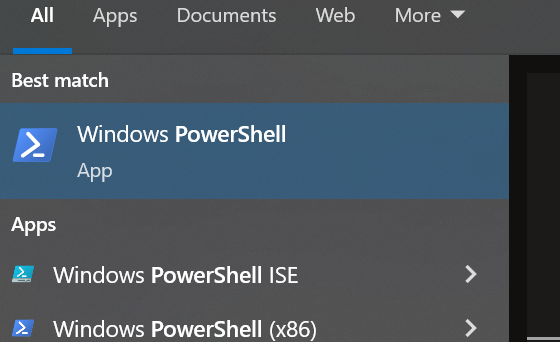
\includegraphics[width=0.5\textwidth,height=0.5\textheight]{images/powershell.png}
\item
  Type \texttt{ssh\ your\_netid@pronto.las.iastate.edu}

  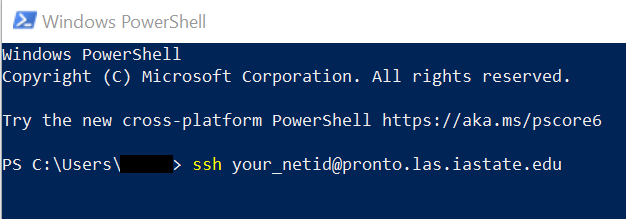
\includegraphics[width=0.5\textwidth,height=0.5\textheight]{images/ssh_to_pronto.png}
\item
  Type your net-id password
\item
  You should now see

\begin{Shaded}
\begin{Highlighting}[]
\ExtensionTok{[your\_netid@pronto}\NormalTok{ \textasciitilde{}]$}
\end{Highlighting}
\end{Shaded}
\end{enumerate}

\textbf{Mac}

\begin{enumerate}
\def\labelenumi{\arabic{enumi}.}
\tightlist
\item
  Do a spotlight search by clicking on the magnifying glass in the upper right corner of the screen

  
\includegraphics[width=0.5\textwidth,height=0.5\textheight]{images/spotlight.png}
\item
  Type \texttt{terminal} and click Terminal in the list

  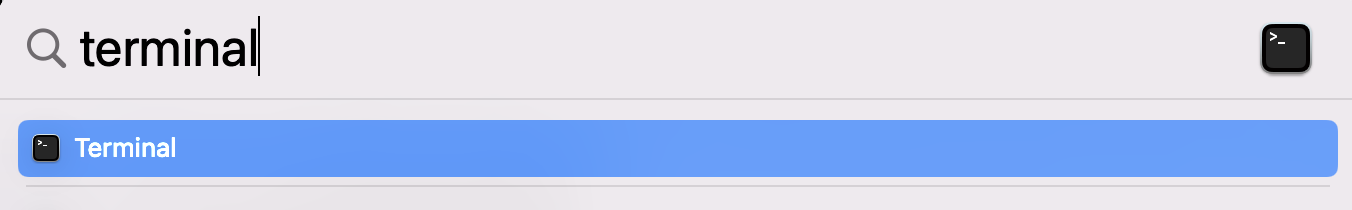
\includegraphics[width=0.5\textwidth,height=0.5\textheight]{images/search_terminal.png}
\item
  In the Terminal widow, type \texttt{ssh\ your\_netid@pronto.las.iastate.edu}

  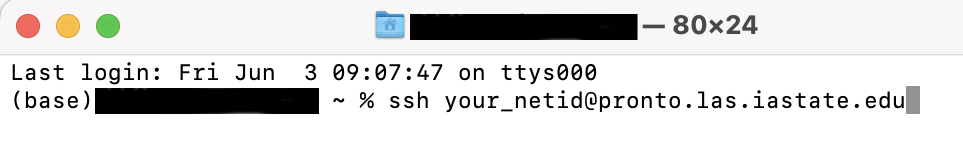
\includegraphics[width=0.5\textwidth,height=0.5\textheight]{images/mac_terminal.png}
\item
  Type your net-id password
\end{enumerate}

\hypertarget{prontodtn}{%
\section{Connecting to the Pronto data transfer node}\label{prontodtn}}

You need to transfer your data to Pronto using the Pronto data transfer node (ProntoDTN). CSAFE has a folder for CSAFE users on ProntoDTN. The file path is \texttt{prontodtn.las.iastate.edu\ \textgreater{}\ work\ \textgreater{}\ LAS\ \textgreater{}\ csafe-lab}. Create a folder for yourself in the csafe-lab folder. Most users use their net-id as the folder name, but I think you can name it anything you want.

The work directory is not backed-up so don't use this folder for long term storage.

Each user also has a home folder. These folders have limited storage so researchIT recommends only placing small files in the home folder. I find it easier to store everything in my work folder and not use my home folder at all.

\textbf{Windows}

\begin{enumerate}
\def\labelenumi{\arabic{enumi}.}
\tightlist
\item
  Open file explorer
\item
  Type \texttt{\textbackslash{}\textbackslash{}prontodtn.las.iastate.edu} in the top textbox

  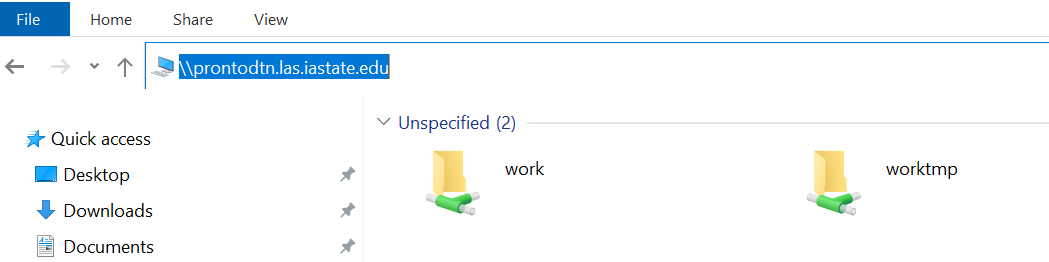
\includegraphics[width=0.5\textwidth,height=0.5\textheight]{images/explorer.png}
\item
  Open the work folder
\item
  Open the LAS folder
\item
  Open the csafe-lab folder
\item
  Create a new folder with your net-id as the name
\end{enumerate}

\textbf{Mac}

\begin{enumerate}
\def\labelenumi{\arabic{enumi}.}
\tightlist
\item
  Select Go \textgreater{} Connect to Server

  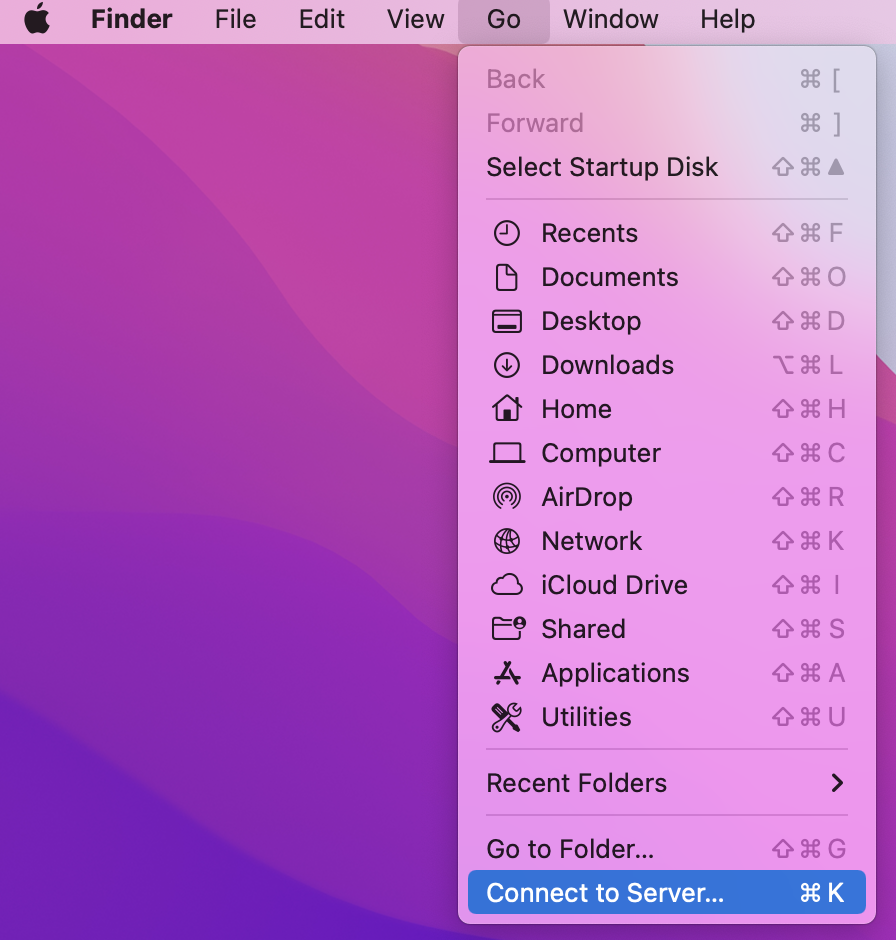
\includegraphics[width=0.5\textwidth,height=0.5\textheight]{images/connect_to_server.png}
\item
  Type \texttt{smb://prontodtn.las.iastate.edu} in the text box. Click the + sign if you would like your computer to remember the server.

  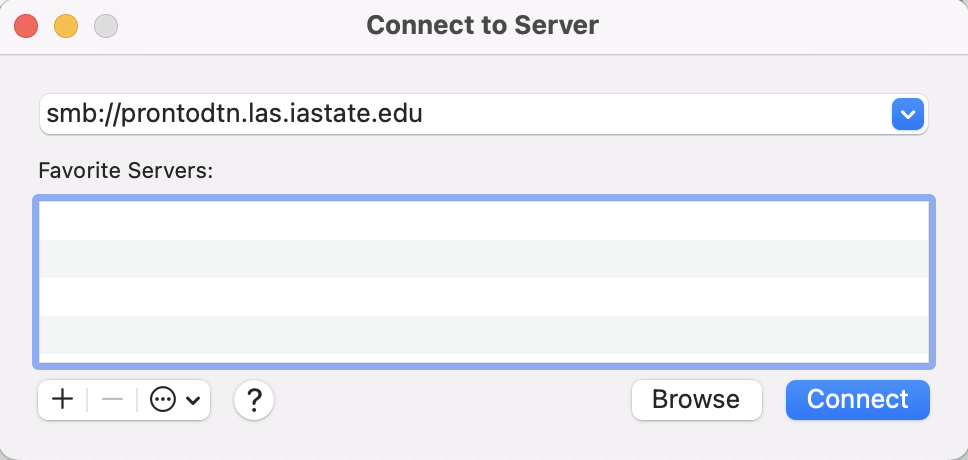
\includegraphics[width=0.5\textwidth,height=0.5\textheight]{images/add_server.png}
\item
  Click Connect
\item
  Enter your net-id and password
\item
  Select Work and click OK.
\item
  Open the LAS folder
\item
  Open the csafe-lab folder
\item
  Create a new folder with your net-id as the name
\end{enumerate}

\hypertarget{transfering-data-from-prontodtn-to-lss}{%
\subsection{Transfering data from ProntoDTN to LSS}\label{transfering-data-from-prontodtn-to-lss}}

\begin{enumerate}
\def\labelenumi{\arabic{enumi}.}
\tightlist
\item
\end{enumerate}

\hypertarget{transfering-large-amounts-of-data-using-globus}{%
\subsection{Transfering large amounts of data using Globus}\label{transfering-large-amounts-of-data-using-globus}}

If you have large amounts of data to transfer, researchIT recommends that you use Globus Connect Personal. Go to \url{https://researchit.las.iastate.edu/how-transfer-files-pronto-globus} to download Globus.

Instructions for transferring data with Globus are here: \url{https://docs.globus.org/how-to/get-started/}.

\hypertarget{running-an-r-script-on-pronto}{%
\section{Running an R script on Pronto}\label{running-an-r-script-on-pronto}}

There are two ways to run a script on Pronto:

\begin{enumerate}
\def\labelenumi{\arabic{enumi}.}
\tightlist
\item
  in an interactive session
\item
  as a batch job
\end{enumerate}

If I understand correctly, an interactive session is intended for troubleshooting your code. ResearchIT says, ``Once you've got your program running in an interactive session please switch to an sbatch script if possible.'' {[}\url{https://researchit.las.iastate.edu/pronto?msclkid=3263c889c17811ec81e13068586d8872}{]}

Pronto uses the Simple Linux Utility for Resource Management (Slurm) to allocate resources (computer nodes and clusters) to users {[}\url{https://en.wikipedia.org/wiki/Slurm_Workload_Manager}{]}. In order to run your script as a batch job, you need to write a Slurm file that includes information about your job and the resources your would like to request.

\hypertarget{interactive-sessions}{%
\section{Interactive Sessions}\label{interactive-sessions}}

\hypertarget{ex-start-interactive}{%
\subsection{Example: Start an interactive session}\label{ex-start-interactive}}

\begin{enumerate}
\def\labelenumi{\arabic{enumi}.}
\item
  If you are off campus, connect to the ISU VPN (see \ref{signin-vpn})
\item
  Sign-in to Pronto (see \ref{pronto}).
\item
  In the Pronto terminal, type

\begin{Shaded}
\begin{Highlighting}[]
\ExtensionTok{$}\NormalTok{ srun }\AttributeTok{{-}{-}nodes}\NormalTok{ 1 }\AttributeTok{{-}{-}tasks}\NormalTok{ 4 }\AttributeTok{{-}{-}partition}\NormalTok{ interactive }\AttributeTok{{-}{-}time}\NormalTok{ 01:00:00 }\AttributeTok{{-}{-}pty}\NormalTok{ bash}
\end{Highlighting}
\end{Shaded}

  This starts an interactive session.
\item
  Load the module for R version 4.0.4. This version of R requires that a specific version of gcc be loaded first.

\begin{Shaded}
\begin{Highlighting}[]
\ExtensionTok{$}\NormalTok{ module load gcc/10.2.0{-}zuvaafu}
\ExtensionTok{$}\NormalTok{ module load r/4.0.4{-}py3{-}4khjixy}
\end{Highlighting}
\end{Shaded}
\item
  Tell Pronto to install R packages in your csafe-lab work folder. (This is considered the best practice by ResearchIT \url{https://researchit.las.iastate.edu/how-run-r-pronto?msclkid=865a487bc65e11ecbfd7e59a7ab1dc47}.)

\begin{Shaded}
\begin{Highlighting}[]
\ExtensionTok{$}\NormalTok{ export R\_LIBS\_USER=/work/LAS/your{-}lab/yournetid/Rlibs}
\ExtensionTok{$}\NormalTok{ mkdir }\AttributeTok{{-}p} \VariableTok{$R\_LIBS\_USER}
\end{Highlighting}
\end{Shaded}
\item
  Start the R interpreter

\begin{Shaded}
\begin{Highlighting}[]
\ExtensionTok{$}\NormalTok{ R}
\end{Highlighting}
\end{Shaded}
\end{enumerate}

\hypertarget{ex-interactive-install}{%
\subsection{Example: Install a package from CRAN}\label{ex-interactive-install}}

\begin{enumerate}
\def\labelenumi{\arabic{enumi}.}
\item
  Start an interactive R session (see \ref{ex-start-interactive})
\item
\begin{Shaded}
\begin{Highlighting}[]
\OperatorTok{\textgreater{}}\NormalTok{ install.packages}\KeywordTok{(}\StringTok{"dplyr"}\ExtensionTok{,lib=}\StringTok{"/work/LAS/csafe{-}lab/your\_netid/Rlibs"}\ExtensionTok{,}\NormalTok{ repos=}\StringTok{"https://mirror.las.iastate.edu/CRAN"}\KeywordTok{)}
\end{Highlighting}
\end{Shaded}
\end{enumerate}

\hypertarget{ex-interactive-install-github}{%
\subsection{Example: Install a package from Github}\label{ex-interactive-install-github}}

Occasionally, you might want to install a package that isn't available on CRAN but is available on GitHub. This example shows how to do that on Pronto.

\begin{enumerate}
\def\labelenumi{\arabic{enumi}.}
\item
  Start an interactive R session (see \ref{ex-start-interactive})
\item
  If you haven't already, you need to install the devtools package

\begin{Shaded}
\begin{Highlighting}[]
\OperatorTok{\textgreater{}}\NormalTok{ install.packages}\KeywordTok{(}\StringTok{"devtools"}\ExtensionTok{,lib=}\StringTok{"/work/LAS/csafe{-}lab/your\_netid/Rlibs"}\ExtensionTok{,}\NormalTok{ repos=}\StringTok{"https://mirror.las.iastate.edu/CRAN"}\KeywordTok{)}
\end{Highlighting}
\end{Shaded}
\item
  Every GitHub repository url has the format \url{https://github.com/GithubUsernam/GithubRepo}. Use the GithubUsername/GithubRepo in the install\_github function.

\begin{Shaded}
\begin{Highlighting}[]
\OperatorTok{\textgreater{}}\NormalTok{ devtools::install\_github}\KeywordTok{(}\StringTok{"GithubUsername/GithubRepo"}\KeywordTok{)}
\end{Highlighting}
\end{Shaded}
\end{enumerate}

\hypertarget{batch-jobs}{%
\section{Batch Jobs}\label{batch-jobs}}

\hypertarget{ex-basic}{%
\subsection{Example: A basic R script}\label{ex-basic}}

\begin{enumerate}
\def\labelenumi{\arabic{enumi}.}
\item
  If you are off campus, connect to the ISU VPN (see \ref{signin-vpn})
\item
  Sign-in to Pronto (see \ref{pronto}).
\item
  Open your csafe-lab work folder \texttt{prontodtn.las.iastate.edu\ \textgreater{}\ work\ \textgreater{}\ LAS\ \textgreater{}\ csafe-lab\ \textgreater{}\ your\_netid} (see \ref{prontodtn})
\item
  Create a new R script with the following lines of code:

\begin{Shaded}
\begin{Highlighting}[]
\NormalTok{a }\OtherTok{=} \DecValTok{5}
\FunctionTok{print}\NormalTok{(a)}
\end{Highlighting}
\end{Shaded}

  Save the script as \texttt{basic.R}. Copy the script to your csafe-lab work folder.
\item
  Create a text file for Slurm with the following text:

\begin{Shaded}
\begin{Highlighting}[]
\CommentTok{\#!/bin/bash}

\CommentTok{\#SBATCH {-}{-}nodes=1 \# request one node}
\CommentTok{\#SBATCH {-}{-}cpus{-}per{-}task=1  \# ask for 1 cpu}
\CommentTok{\#SBATCH {-}{-}mem=1G \#  asks for 1 GB of RAM}
\CommentTok{\#SBATCH {-}{-}time=00:30:02 \# ask that the job be allowed to run for 30 minutes and 2 seconds.}

\CommentTok{\# everything below this line is optional}
\CommentTok{\#SBATCH {-}{-}output=/work/LAS/csafe{-}lab/your\_netid/job\_\%J\_out.txt \# store console output}
\CommentTok{\#SBATCH {-}{-}error=/work/LAS/csafe{-}lab/your\_netid/job\_\%J\_err.txt \# store error messages}

\ExtensionTok{module}\NormalTok{ load r}
\BuiltInTok{cd}\NormalTok{ /work/LAS/csafe{-}lab/your\_netid}
\ExtensionTok{R} \AttributeTok{{-}{-}save} \OperatorTok{\textless{}}\NormalTok{ basic.R}
\end{Highlighting}
\end{Shaded}

  Save the file as \texttt{basic.txt}.
\item
  (Windows Only) If you are using Windows, your text file will likely have DOS line breaks instead of UNIX line breaks which will cause an error when the file is run on Pronto. Open Terminal in RStudio, use \texttt{cd\ folder/containing/text\_file} to change directories to the folder containing your text file, and type \texttt{dos2unix\ basic.txt} to change the line breaks to UNIX format.
\item
  Copy the text file to your csafe-lab work folder.
\item
  In the command line prompt where you are connected to Pronto, type

\begin{Shaded}
\begin{Highlighting}[]
\ExtensionTok{$}\NormalTok{ sbatch /work/LAS/csafe{-}lab/your\_netid/basic.txt}
\end{Highlighting}
\end{Shaded}

  This will add your job to the queue. The script is so short, your job will probably run immediately.
\item
  Two new files -- \texttt{job\_\textless{}job\#\textgreater{}\_err.txt} and \texttt{job\_\textless{}job\#\textgreater{}\_out.txt} -- should appear in your csafe-lab work folder. If \texttt{basic.R} ran successfully, the \texttt{job\_\textless{}job\#\textgreater{}\_out} file should contain

\begin{Shaded}
\begin{Highlighting}[]
\OperatorTok{\textgreater{}}\NormalTok{ a }\ExtensionTok{=}\NormalTok{ 5}
\OperatorTok{\textgreater{}}\NormalTok{ print}\KeywordTok{(}\ExtensionTok{a}\KeywordTok{)}
\ExtensionTok{[1]}\NormalTok{ 5}
\OperatorTok{\textgreater{}} 
\end{Highlighting}
\end{Shaded}

  and \texttt{job\_\textless{}job\#\textgreater{}\_err.txt} should be blank. If the error file isn't blank, troubleshoot the error(s). If you get stuck, email \href{mailto:researchit@iastate.edu}{\nolinkurl{researchit@iastate.edu}}.
\end{enumerate}

\hypertarget{ex-save}{%
\subsection{Example: Save a dataframe to a CSV file}\label{ex-save}}

In this example, I will show you how to save a dataframe to a csv file.

\begin{enumerate}
\def\labelenumi{\arabic{enumi}.}
\item
  If you are off campus, connect to the ISU VPN (see \ref{signin-vpn})
\item
  Sign-in to Pronto (see \ref{pronto}).
\item
  Open your csafe-lab work folder \texttt{prontodtn.las.iastate.edu\ \textgreater{}\ work\ \textgreater{}\ LAS\ \textgreater{}\ csafe-lab\ \textgreater{}\ your\_netid} (see \ref{prontodtn})
\item
  Create a new R script with the following lines of code:

\begin{Shaded}
\begin{Highlighting}[]
\CommentTok{\# draw 10 samples from normal distribution}
\NormalTok{data }\OtherTok{=} \FunctionTok{rnorm}\NormalTok{(}\DecValTok{10}\NormalTok{)}

\CommentTok{\# put in a dataframe}
\NormalTok{df }\OtherTok{=} \FunctionTok{data.frame}\NormalTok{(}\AttributeTok{x=}\NormalTok{data)}

\CommentTok{\# save dataframe}
\FunctionTok{write.csv}\NormalTok{(df, }\StringTok{"data.csv"}\NormalTok{)}
\end{Highlighting}
\end{Shaded}

  Save the script as \texttt{dataframe.R}. Copy the script to your csafe-lab work folder.
\item
  Create a text file for Slurm with the following text:

\begin{Shaded}
\begin{Highlighting}[]
\CommentTok{\#!/bin/bash}

\CommentTok{\#SBATCH {-}{-}nodes=1 \# request one node}
\CommentTok{\#SBATCH {-}{-}cpus{-}per{-}task=1  \# ask for 1 cpu}
\CommentTok{\#SBATCH {-}{-}mem=1G \#  asks for 1 GB of RAM}
\CommentTok{\#SBATCH {-}{-}time=00:30:02 \# ask that the job be allowed to run for 30 minutes and 2 seconds.}

\CommentTok{\# everything below this line is optional}
\CommentTok{\#SBATCH {-}{-}output=/work/LAS/csafe{-}lab/your\_netid/job\_\%J\_out.txt \# store console output}
\CommentTok{\#SBATCH {-}{-}error=/work/LAS/csafe{-}lab/your\_netid/job\_\%J\_err.txt \# store error messages}

\ExtensionTok{module}\NormalTok{ load r}
\BuiltInTok{cd}\NormalTok{ /work/LAS/csafe{-}lab/your\_netid}
\ExtensionTok{R} \AttributeTok{{-}{-}save} \OperatorTok{\textless{}}\NormalTok{ dataframe.R}
\end{Highlighting}
\end{Shaded}

  Save the file as \texttt{dataframe.txt}.
\item
  (Windows Only) If you are using Windows, your text file will likely have DOS line breaks instead of UNIX line breaks which will cause an error when the file is run on Pronto. Open Terminal in RStudio, use \texttt{cd\ folder/containing/text\_file} to change directories to the folder containing your text file, and type \texttt{dos2unix\ dataframe.txt} to change the line breaks to UNIX format.
\item
  Copy the text file to your csafe-lab work folder.
\item
  In the command line prompt where you are connected to Pronto, type

\begin{Shaded}
\begin{Highlighting}[]
\ExtensionTok{$}\NormalTok{ sbatch /work/LAS/csafe{-}lab/your\_netid/dataframe.txt}
\end{Highlighting}
\end{Shaded}

  This will add your job to the queue. The script is so short, your job will probably run immediately.
\item
  The dataframe should be saved in a file \texttt{data.csv} in your csafe-lab work folder. There should be two other new files -- \texttt{data.csv}, \texttt{job\_\textless{}job\#\textgreater{}\_err.txt} and \texttt{job\_\textless{}job\#\textgreater{}\_out.txt} -- in your csafe-lab work folder as well. If the error file isn't blank, troubleshoot the error(s). If you get stuck, email \href{mailto:researchit@iastate.edu}{\nolinkurl{researchit@iastate.edu}}.
\end{enumerate}

\hypertarget{ex-load}{%
\subsection{Example: Load data from a CSV file}\label{ex-load}}

In this example, we will load the csv file \texttt{data.csv} that we saved in Example \ref{ex-save}.

\begin{enumerate}
\def\labelenumi{\arabic{enumi}.}
\item
  If you are off campus, connect to the ISU VPN (see \ref{signin-vpn})
\item
  Sign-in to Pronto (see \ref{pronto}).
\item
  Open your csafe-lab work folder \texttt{prontodtn.las.iastate.edu\ \textgreater{}\ work\ \textgreater{}\ LAS\ \textgreater{}\ csafe-lab\ \textgreater{}\ your\_netid} (see \ref{prontodtn})
\item
  Double-check that the file \texttt{data.csv} is still in your csafe-lab work folder. If you deleted it, follow the steps in example \ref{ex-save} to recreate it.
\item
  Create a new R script with the following lines of code:

\begin{Shaded}
\begin{Highlighting}[]
\NormalTok{df }\OtherTok{=} \FunctionTok{read.csv}\NormalTok{(}\StringTok{"data.csv"}\NormalTok{)}
\FunctionTok{head}\NormalTok{(df)}
\end{Highlighting}
\end{Shaded}

  Save the script as \texttt{load.R} and copy it to you csafe-lab work folder.
\item
  Create a text file for Slurm with the following text:

\begin{Shaded}
\begin{Highlighting}[]
\CommentTok{\#!/bin/bash}

\CommentTok{\#SBATCH {-}{-}nodes=1 \# request one node}
\CommentTok{\#SBATCH {-}{-}cpus{-}per{-}task=1  \# ask for 1 cpu}
\CommentTok{\#SBATCH {-}{-}mem=1G \#  asks for 1 GB of RAM}
\CommentTok{\#SBATCH {-}{-}time=00:30:02 \# ask that the job be allowed to run for 30 minutes and 2 seconds.}

\CommentTok{\# everything below this line is optional}
\CommentTok{\#SBATCH {-}{-}output=/work/LAS/csafe{-}lab/your\_netid/job\_\%J\_out.txt \# store console output}
\CommentTok{\#SBATCH {-}{-}error=/work/LAS/csafe{-}lab/your\_netid/job\_\%J\_err.txt \# store error messages}

\ExtensionTok{module}\NormalTok{ load r}
\BuiltInTok{cd}\NormalTok{ /work/LAS/csafe{-}lab/your\_netid}
\ExtensionTok{R} \AttributeTok{{-}{-}save} \OperatorTok{\textless{}}\NormalTok{ load.R}
\end{Highlighting}
\end{Shaded}

  Save the file as \texttt{load.txt}.
\item
  (Windows Only) If you are using Windows, your text file will likely have DOS line breaks instead of UNIX line breaks which will cause an error when the file is run on Pronto. Open Terminal in RStudio, use \texttt{cd\ folder/containing/text\_file} to change directories to the folder containing your text file, and type \texttt{dos2unix\ load.txt} to change the line breaks to UNIX format.
\item
  Copy the text file to your csafe-lab work folder.
\item
  In the command line prompt where you are connected to Pronto, type

\begin{Shaded}
\begin{Highlighting}[]
\ExtensionTok{$}\NormalTok{ sbatch /work/LAS/csafe{-}lab/your\_netid/load.txt}
\end{Highlighting}
\end{Shaded}

  This will add your job to the queue. The script is so short, your job will probably run immediately.
\item
  Open the file \texttt{job\_\textless{}job\#\textgreater{}\_out.txt} in your csafe-lab work folder and make sure that the first six lines of the dataframe were printed.
\end{enumerate}

\hypertarget{ex-batch-install}{%
\subsection{Example: Install R packages}\label{ex-batch-install}}

Just like in Rstudio on your local machine, you will need to install any R packages that you want use. In this example, we will install futile.logger, doParallel, doRNG, and tidyverse so that we can use these packages in future examples.

\begin{enumerate}
\def\labelenumi{\arabic{enumi}.}
\item
  If you are off campus, connect to the ISU VPN (see \ref{signin-vpn})
\item
  Sign-in to Pronto (see \ref{pronto}).
\item
  Open your csafe-lab work folder \texttt{prontodtn.las.iastate.edu\ \textgreater{}\ work\ \textgreater{}\ LAS\ \textgreater{}\ csafe-lab\ \textgreater{}\ your\_netid} (see \ref{prontodtn})
\item
  Create a new R script with the following lines of code:

\begin{Shaded}
\begin{Highlighting}[]
\FunctionTok{install.packages}\NormalTok{(}\FunctionTok{c}\NormalTok{(}\StringTok{"futile.logger"}\NormalTok{, }
                   \StringTok{"doParallel"}\NormalTok{, }
                   \StringTok{"doRNG"}\NormalTok{,}
                   \StringTok{"tidyverse"}\NormalTok{), }
                   \AttributeTok{lib=}\StringTok{"/work/LAS/csafe{-}lab/your\_netid/Rlibs"}\NormalTok{, }
                   \AttributeTok{repos=}\StringTok{"https://mirror.las.iastate.edu/CRAN"}\NormalTok{)}
\end{Highlighting}
\end{Shaded}

  The line starting with \texttt{lib=} tells Pronto to install the R packages in your csafe-lab work folder. The line starting with \texttt{repos=} tells Pronto which CRAN mirror to use. ResearchIT says that these two lines should always be used {[}\url{https://researchit.las.iastate.edu/how-run-r-pronto}{]}. Save the script as \texttt{install\_packages.R}. Copy the script to your csafe-lab work folder.
\item
  Create a text file for Slurm with the following text:

\begin{Shaded}
\begin{Highlighting}[]
\CommentTok{\#!/bin/bash}

\CommentTok{\#SBATCH {-}{-}nodes=1 \# request one node}
\CommentTok{\#SBATCH {-}{-}cpus{-}per{-}task=1  \# ask for 1 cpu}
\CommentTok{\#SBATCH {-}{-}mem=1G \#  asks for 1 GB of RAM}
\CommentTok{\#SBATCH {-}{-}time=00:30:02 \# ask that the job be allowed to run for 30 minutes and 2 seconds.}

\CommentTok{\# everything below this line is optional}
\CommentTok{\#SBATCH {-}{-}output=/work/LAS/csafe{-}lab/your\_netid/job\_\%J\_out.txt \# store console output}
\CommentTok{\#SBATCH {-}{-}error=/work/LAS/csafe{-}lab/your\_netid/job\_\%J\_err.txt \# store error messages}

\BuiltInTok{export} \VariableTok{R\_LIBS\_USER}\OperatorTok{=}\NormalTok{/work/LAS/csafe{-}lab/your\_netid/Rlibs}
\FunctionTok{mkdir} \AttributeTok{{-}p} \VariableTok{$R\_LIBS\_USER}

\ExtensionTok{module}\NormalTok{ load r}
\BuiltInTok{cd}\NormalTok{ /work/LAS/csafe{-}lab/your\_netid}
\ExtensionTok{R} \AttributeTok{{-}{-}save} \OperatorTok{\textless{}}\NormalTok{ install\_packages.R}
\end{Highlighting}
\end{Shaded}

  Save the file as \texttt{install\_packages.txt}.
\item
  (Windows Only) If you are using Windows, your text file will likely have DOS line breaks instead of UNIX line breaks which will cause an error when the file is run on Pronto. Open Terminal in RStudio, use \texttt{cd\ folder/containing/text\_file} to change directories to the folder containing your text file, and type \texttt{dos2unix\ install\_packages.txt} to change the line breaks to UNIX format.
\item
  Copy the text file to your csafe-lab work folder.
\item
  In the command line prompt where you are connected to Pronto, type

\begin{Shaded}
\begin{Highlighting}[]
\ExtensionTok{$}\NormalTok{ sbatch /work/LAS/csafe{-}lab/your\_netid/install\_packages.txt}
\end{Highlighting}
\end{Shaded}

  This will add your job to the queue. Just like on your local machine, it might take several minutes to install the packages.
\item
  There should be two other new files -- \texttt{data.csv}, \texttt{job\_\textless{}job\#\textgreater{}\_err.txt} and \texttt{job\_\textless{}job\#\textgreater{}\_out.txt} -- in your csafe-lab work folder.
\end{enumerate}

\hypertarget{ex-parallel}{%
\subsection{Example: Run code in parallel}\label{ex-parallel}}

The main benefit of Pronto is that it can run code in parallel. In this example, I will show you how to run a for loop in parallel using the doParallel library. R has other packages for parallel computing, but ResearchIT uses doParallel in their how-to {[}\url{https://researchit.las.iastate.edu/how-run-r-pronto}{]} so that's what I will use here.

If you completed Example \ref{ex-batch-install} the doParallel package will already be installed. If you need to install the doParallel package see Examples \ref{ex-interactive-install} or \ref{ex-batch-install} for instructions.

\begin{enumerate}
\def\labelenumi{\arabic{enumi}.}
\item
  If you are off campus, connect to the ISU VPN (see \ref{signin-vpn})
\item
  Sign-in to Pronto (see \ref{pronto}).
\item
  Open your csafe-lab work folder \texttt{prontodtn.las.iastate.edu\ \textgreater{}\ work\ \textgreater{}\ LAS\ \textgreater{}\ csafe-lab\ \textgreater{}\ your\_netid} (see \ref{prontodtn})
\item
  Create a new R script with the following lines of code:

\begin{Shaded}
\begin{Highlighting}[]
\FunctionTok{library}\NormalTok{(doParallel)}

\NormalTok{nCores }\OtherTok{=} \FunctionTok{as.integer}\NormalTok{(}\FunctionTok{Sys.getenv}\NormalTok{(}\StringTok{"SLURM\_CPUS\_PER\_TASK"}\NormalTok{))}
\NormalTok{myCluster }\OtherTok{=}\NormalTok{ parallel}\SpecialCharTok{::}\FunctionTok{makeCluster}\NormalTok{(nCores)}
\NormalTok{doParallel}\SpecialCharTok{::}\FunctionTok{registerDoParallel}\NormalTok{(myCluster)}

\NormalTok{results }\OtherTok{=} \FunctionTok{foreach}\NormalTok{(}\AttributeTok{i=}\DecValTok{1}\SpecialCharTok{:}\DecValTok{10}\NormalTok{) }\SpecialCharTok{\%dopar\%}\NormalTok{ \{}
  \FunctionTok{rnorm}\NormalTok{(}\DecValTok{1000}\NormalTok{)\}}
\FunctionTok{saveRDS}\NormalTok{(results, }\StringTok{"parallel\_results.rds"}\NormalTok{)}
\end{Highlighting}
\end{Shaded}

  Save the script as \texttt{parallel.R}. Copy the script to your csafe-lab work folder.
\item
  Create a text file for Slurm with the following text:

\begin{Shaded}
\begin{Highlighting}[]
\CommentTok{\#!/bin/bash}

\CommentTok{\#SBATCH {-}{-}nodes=1 \# request one node}
\CommentTok{\#SBATCH {-}{-}cpus{-}per{-}task=10  \# ask for 10 cpu}
\CommentTok{\#SBATCH {-}{-}mem=1G \#  asks for 1 GB of RAM}
\CommentTok{\#SBATCH {-}{-}time=00:30:02 \# ask that the job be allowed to run for 30 minutes and 2 seconds.}

\CommentTok{\# everything below this line is optional}
\CommentTok{\#SBATCH {-}{-}output=/work/LAS/csafe{-}lab/your\_netid/job\_\%J\_out.txt \# store console output}
\CommentTok{\#SBATCH {-}{-}error=/work/LAS/csafe{-}lab/your\_netid/job\_\%J\_err.txt \# store error messages}

\BuiltInTok{export} \VariableTok{R\_LIBS\_USER}\OperatorTok{=}\NormalTok{/work/LAS/csafe{-}lab/your\_netid/Rlibs}

\ExtensionTok{module}\NormalTok{ load r}
\BuiltInTok{cd}\NormalTok{ /work/LAS/csafe{-}lab/your\_netid}
\ExtensionTok{R} \AttributeTok{{-}{-}save} \OperatorTok{\textless{}}\NormalTok{ parallel.R}
\end{Highlighting}
\end{Shaded}

  Save the file as \texttt{parallel.txt}.
\item
  (Windows Only) If you are using Windows, your text file will likely have DOS line breaks instead of UNIX line breaks which will cause an error when the file is run on Pronto. Open Terminal in RStudio, use \texttt{cd\ folder/containing/text\_file} to change directories to the folder containing your text file, and type \texttt{dos2unix\ parallel.txt} to change the line breaks to UNIX format.
\item
  Copy the text file to your csafe-lab work folder.
\item
  In the command line prompt where you are connected to Pronto, type

\begin{Shaded}
\begin{Highlighting}[]
\ExtensionTok{$}\NormalTok{ sbatch /work/LAS/csafe{-}lab/your\_netid/parallel.txt}
\end{Highlighting}
\end{Shaded}
\item
  The results of the parallel loop should be saved in \texttt{parallel.txt} in your csafe-lab work folder.
\end{enumerate}

\hypertarget{ex-seed}{%
\subsection{Example: Set the seed for the random number generator}\label{ex-seed}}

If you run Example \ref{ex-parallel} multiple times, the numbers sampled from the normal distribution will likely be different each time. If you want to make the sample reproducible
(produce the same sample each time), set the seed for the random number generator. The most common way to set a seed is with the \texttt{set.seed()} function. This function does not work with \texttt{\%dopar\%} from the doParallel package, but it does work with \texttt{\%dorng\%}.

\begin{enumerate}
\def\labelenumi{\arabic{enumi}.}
\item
  If you are off campus, connect to the ISU VPN (see \ref{signin-vpn})
\item
  Sign-in to Pronto (see \ref{pronto}).
\item
  Open your csafe-lab work folder \texttt{prontodtn.las.iastate.edu\ \textgreater{}\ work\ \textgreater{}\ LAS\ \textgreater{}\ csafe-lab\ \textgreater{}\ your\_netid} (see \ref{prontodtn})
\item
  Create a new R script with the following lines of code:

\begin{Shaded}
\begin{Highlighting}[]
\FunctionTok{library}\NormalTok{(doParallel)}
\FunctionTok{library}\NormalTok{(doRNG)}

\NormalTok{nCores }\OtherTok{=} \FunctionTok{as.integer}\NormalTok{(}\FunctionTok{Sys.getenv}\NormalTok{(}\StringTok{"SLURM\_CPUS\_PER\_TASK"}\NormalTok{))}
\NormalTok{myCluster }\OtherTok{=}\NormalTok{ parallel}\SpecialCharTok{::}\FunctionTok{makeCluster}\NormalTok{(nCores)}
\NormalTok{doParallel}\SpecialCharTok{::}\FunctionTok{registerDoParallel}\NormalTok{(myCluster)}

\NormalTok{starting\_seed }\OtherTok{=} \DecValTok{300}

\FunctionTok{set.seed}\NormalTok{(starting\_seed)}
\NormalTok{r1 }\OtherTok{=} \FunctionTok{foreach}\NormalTok{(}\AttributeTok{i=}\DecValTok{1}\SpecialCharTok{:}\DecValTok{4}\NormalTok{) }\SpecialCharTok{\%dorng\%}\NormalTok{\{ }\FunctionTok{runif}\NormalTok{(}\DecValTok{1}\NormalTok{) \}}

\FunctionTok{set.seed}\NormalTok{(starting\_seed)}
\NormalTok{r2 }\OtherTok{=} \FunctionTok{foreach}\NormalTok{(}\AttributeTok{i=}\DecValTok{1}\SpecialCharTok{:}\DecValTok{4}\NormalTok{) }\SpecialCharTok{\%dorng\%}\NormalTok{\{ }\FunctionTok{runif}\NormalTok{(}\DecValTok{1}\NormalTok{) \}}
\FunctionTok{identical}\NormalTok{(r1, r2)}
\end{Highlighting}
\end{Shaded}

  Save the script as \texttt{seed.R}. Copy the script to your csafe-lab work folder.
\item
  Create a text file for Slurm with the following text:

\begin{Shaded}
\begin{Highlighting}[]
\CommentTok{\#!/bin/bash}

\CommentTok{\#SBATCH {-}{-}nodes=1 \# request one node}
\CommentTok{\#SBATCH {-}{-}cpus{-}per{-}task=10  \# ask for 10 cpu}
\CommentTok{\#SBATCH {-}{-}mem=1G \#  asks for 1 GB of RAM}
\CommentTok{\#SBATCH {-}{-}time=00:30:02 \# ask that the job be allowed to run for 30 minutes and 2 seconds.}

\CommentTok{\# everything below this line is optional}
\CommentTok{\#SBATCH {-}{-}output=/work/LAS/csafe{-}lab/your\_netid/job\_\%J\_out.txt \# store console output}
\CommentTok{\#SBATCH {-}{-}error=/work/LAS/csafe{-}lab/your\_netid/job\_\%J\_err.txt \# store error messages}

\BuiltInTok{export} \VariableTok{R\_LIBS\_USER}\OperatorTok{=}\NormalTok{/work/LAS/csafe{-}lab/your\_netid/Rlibs}

\ExtensionTok{module}\NormalTok{ load r}
\BuiltInTok{cd}\NormalTok{ /work/LAS/csafe{-}lab/your\_netid}
\ExtensionTok{R} \AttributeTok{{-}{-}save} \OperatorTok{\textless{}}\NormalTok{ seed.R}
\end{Highlighting}
\end{Shaded}

  Save the file as \texttt{seed.txt}.
\item
  (Windows Only) If you are using Windows, your text file will likely have DOS line breaks instead of UNIX line breaks which will cause an error when the file is run on Pronto. Open Terminal in RStudio, use \texttt{cd\ folder/containing/text\_file} to change directories to the folder containing your text file, and type \texttt{dos2unix\ seed.txt} to change the line breaks to UNIX format.
\item
  Copy the text file to your csafe-lab work folder.
\item
  In the command line prompt where you are connected to Pronto, type

\begin{Shaded}
\begin{Highlighting}[]
\ExtensionTok{$}\NormalTok{ sbatch /work/LAS/csafe{-}lab/your\_netid/seed.txt}
\end{Highlighting}
\end{Shaded}
\item
  Open the \texttt{job\_\textless{}job\#\textgreater{}\_out.txt} file to make sure that the result of \texttt{identical(r1,\ r2)} is \texttt{TRUE}.
\end{enumerate}

\hypertarget{ex-packages-parallel}{%
\subsection{Example: Use functions from dplyr and magrittr in parallel}\label{ex-packages-parallel}}

The previous parallel examples used the base R functions \texttt{rnorm} and \texttt{runif}. If we want to use
functions from packages that we install, we need to pass the package names to the \texttt{\%dorng\%} operator. We will learn how to do this in this example.

If you haven't already installed the \texttt{tidyverse} package, follow the steps in Example 4 to install the \texttt{tidyverse} or install \texttt{dplyr} and \texttt{magrittr} separately.

\begin{enumerate}
\def\labelenumi{\arabic{enumi}.}
\item
  If you are off campus, connect to the ISU VPN (see \ref{signin-vpn})
\item
  Sign-in to Pronto (see \ref{pronto}).
\item
  Open your csafe-lab work folder \texttt{prontodtn.las.iastate.edu\ \textgreater{}\ work\ \textgreater{}\ LAS\ \textgreater{}\ csafe-lab\ \textgreater{}\ your\_netid} (see \ref{prontodtn})
\item
  Create a new R script with the following lines of code:

\begin{Shaded}
\begin{Highlighting}[]
\FunctionTok{library}\NormalTok{(doParallel)}
\FunctionTok{library}\NormalTok{(doRNG)}
\FunctionTok{library}\NormalTok{(magrittr)}
\FunctionTok{library}\NormalTok{(dplyr)}

\NormalTok{nCores }\OtherTok{=} \FunctionTok{as.integer}\NormalTok{(}\FunctionTok{Sys.getenv}\NormalTok{(}\StringTok{"SLURM\_CPUS\_PER\_TASK"}\NormalTok{))}
\NormalTok{myCluster }\OtherTok{=}\NormalTok{ parallel}\SpecialCharTok{::}\FunctionTok{makeCluster}\NormalTok{(nCores)}
\NormalTok{doParallel}\SpecialCharTok{::}\FunctionTok{registerDoParallel}\NormalTok{(myCluster)}

\FunctionTok{set.seed}\NormalTok{(}\DecValTok{100}\NormalTok{)}
\NormalTok{r1 }\OtherTok{=} \FunctionTok{foreach}\NormalTok{(}\AttributeTok{i=}\DecValTok{1}\SpecialCharTok{:}\DecValTok{10}\NormalTok{, }\AttributeTok{.packages=}\FunctionTok{c}\NormalTok{(}\StringTok{"dplyr"}\NormalTok{, }\StringTok{"magrittr"}\NormalTok{)) }\SpecialCharTok{\%dorng\%}\NormalTok{\{ }
\NormalTok{  cluster\_centers }\OtherTok{=}\NormalTok{ df }\SpecialCharTok{\%\textgreater{}\%} \FunctionTok{slice\_sample}\NormalTok{(}\AttributeTok{n=}\DecValTok{40}\NormalTok{)}
\NormalTok{\}}

\FunctionTok{set.seed}\NormalTok{(}\DecValTok{100}\NormalTok{)}
\NormalTok{r2 }\OtherTok{=} \FunctionTok{foreach}\NormalTok{(}\AttributeTok{i=}\DecValTok{1}\SpecialCharTok{:}\DecValTok{10}\NormalTok{, }\AttributeTok{.packages=}\FunctionTok{c}\NormalTok{(}\StringTok{"dplyr"}\NormalTok{, }\StringTok{"magrittr"}\NormalTok{)) }\SpecialCharTok{\%dorng\%}\NormalTok{\{ }
\NormalTok{  cluster\_centers }\OtherTok{=}\NormalTok{ df }\SpecialCharTok{\%\textgreater{}\%} \FunctionTok{slice\_sample}\NormalTok{(}\AttributeTok{n=}\DecValTok{40}\NormalTok{)}
\NormalTok{\}}

\FunctionTok{set.seed}\NormalTok{(}\DecValTok{200}\NormalTok{)}
\NormalTok{r3 }\OtherTok{=} \FunctionTok{foreach}\NormalTok{(}\AttributeTok{i=}\DecValTok{1}\SpecialCharTok{:}\DecValTok{10}\NormalTok{, }\AttributeTok{.packages=}\FunctionTok{c}\NormalTok{(}\StringTok{"dplyr"}\NormalTok{, }\StringTok{"magrittr"}\NormalTok{)) }\SpecialCharTok{\%dorng\%}\NormalTok{\{ }
\NormalTok{  cluster\_centers }\OtherTok{=}\NormalTok{ df }\SpecialCharTok{\%\textgreater{}\%} \FunctionTok{slice\_sample}\NormalTok{(}\AttributeTok{n=}\DecValTok{40}\NormalTok{)}
\NormalTok{\}}

\FunctionTok{identical}\NormalTok{(r1, r2)}
\FunctionTok{identical}\NormalTok{(r1, r3)}
\end{Highlighting}
\end{Shaded}

  Save the script as \texttt{magrittr.R}. Copy the script to your csafe-lab work folder.
\item
  Create a text file for Slurm with the following text:

\begin{Shaded}
\begin{Highlighting}[]
\CommentTok{\#!/bin/bash}

\CommentTok{\#SBATCH {-}{-}nodes=1 \# request one node}
\CommentTok{\#SBATCH {-}{-}cpus{-}per{-}task=10  \# ask for 10 cpu}
\CommentTok{\#SBATCH {-}{-}mem=1G \#  asks for 1 GB of RAM}
\CommentTok{\#SBATCH {-}{-}time=00:30:02 \# ask that the job be allowed to run for 30 minutes and 2 seconds.}

\CommentTok{\# everything below this line is optional}
\CommentTok{\#SBATCH {-}{-}output=/work/LAS/csafe{-}lab/your\_netid/job\_\%J\_out.txt \# store console output}
\CommentTok{\#SBATCH {-}{-}error=/work/LAS/csafe{-}lab/your\_netid/job\_\%J\_err.txt \# store error messages}

\BuiltInTok{export} \VariableTok{R\_LIBS\_USER}\OperatorTok{=}\NormalTok{/work/LAS/csafe{-}lab/your\_netid/Rlibs}

\ExtensionTok{module}\NormalTok{ load r}
\BuiltInTok{cd}\NormalTok{ /work/LAS/csafe{-}lab/your\_netid}
\ExtensionTok{R} \AttributeTok{{-}{-}save} \OperatorTok{\textless{}}\NormalTok{ magrittr.R}
\end{Highlighting}
\end{Shaded}

  Save the file as \texttt{magrittr.txt}.
\item
  (Windows Only) If you are using Windows, your text file will likely have DOS line breaks instead of UNIX line breaks which will cause an error when the file is run on Pronto. Open Terminal in RStudio, use \texttt{cd\ folder/containing/text\_file} to change directories to the folder containing your text file, and type \texttt{dos2unix\ magrittr.txt} to change the line breaks to UNIX format.
\item
  Copy the text file to your csafe-lab work folder.
\item
  In the command line prompt where you are connected to Pronto, type

\begin{Shaded}
\begin{Highlighting}[]
\ExtensionTok{$}\NormalTok{ sbatch /work/LAS/csafe{-}lab/your\_netid/magrittr.txt}
\end{Highlighting}
\end{Shaded}
\item
  Open the \texttt{job\_\textless{}job\#\textgreater{}\_out.txt} file to make sure that the result of \texttt{identical(r1,\ r2)} is \texttt{TRUE} and \texttt{identical(r1,\ r3)} is \texttt{FALSE}.
\end{enumerate}

\hypertarget{example-use-a-user-defined-function-to-save-results-inside-a-parallel-loop}{%
\subsection{Example: Use a user-defined function to save results inside a parallel loop}\label{example-use-a-user-defined-function-to-save-results-inside-a-parallel-loop}}

\begin{enumerate}
\def\labelenumi{\arabic{enumi}.}
\item
  If you are off campus, connect to the ISU VPN (see \ref{signin-vpn})
\item
  Sign-in to Pronto (see \ref{pronto}).
\item
  Open your csafe-lab work folder \texttt{prontodtn.las.iastate.edu\ \textgreater{}\ work\ \textgreater{}\ LAS\ \textgreater{}\ csafe-lab\ \textgreater{}\ your\_netid} (see \ref{prontodtn})
\item
  Create a new R script with the following lines of code:

\begin{Shaded}
\begin{Highlighting}[]
\FunctionTok{library}\NormalTok{(doParallel)}
\FunctionTok{library}\NormalTok{(doRNG)}
\FunctionTok{source}\NormalTok{(}\StringTok{"parallel\_save.R"}\NormalTok{)}

\NormalTok{nCores }\OtherTok{=} \FunctionTok{as.integer}\NormalTok{(}\FunctionTok{Sys.getenv}\NormalTok{(}\StringTok{"SLURM\_CPUS\_PER\_TASK"}\NormalTok{))}
\NormalTok{myCluster }\OtherTok{=}\NormalTok{ parallel}\SpecialCharTok{::}\FunctionTok{makeCluster}\NormalTok{(nCores)}
\NormalTok{doParallel}\SpecialCharTok{::}\FunctionTok{registerDoParallel}\NormalTok{(myCluster)}

\NormalTok{starting\_seed }\OtherTok{=} \DecValTok{300}

\FunctionTok{set.seed}\NormalTok{(starting\_seed)}
\NormalTok{r1 }\OtherTok{=} \FunctionTok{foreach}\NormalTok{(}\AttributeTok{i=}\DecValTok{1}\SpecialCharTok{:}\DecValTok{10}\NormalTok{) }\SpecialCharTok{\%dorng\%}\NormalTok{ \{}
  \FunctionTok{save\_sample}\NormalTok{(}\AttributeTok{n=}\DecValTok{10000}\NormalTok{, }\AttributeTok{filename=}\FunctionTok{paste0}\NormalTok{(}\StringTok{"sample\_"}\NormalTok{,i,}\StringTok{".rds"}\NormalTok{)) }
\NormalTok{\}}
\end{Highlighting}
\end{Shaded}

  Save the script as \texttt{run\_parallel\_save.R}. Copy the script to your csafe-lab work folder.
\item
  Create a text file for Slurm with the following text:

\begin{Shaded}
\begin{Highlighting}[]
\CommentTok{\#!/bin/bash}

\CommentTok{\#SBATCH {-}{-}nodes=1 \# request one node}
\CommentTok{\#SBATCH {-}{-}cpus{-}per{-}task=10}
\CommentTok{\#SBATCH {-}{-}mem=2G }
\CommentTok{\#SBATCH {-}{-}time=00:15:00}

\CommentTok{\# everything below this line is optional}
\CommentTok{\#SBATCH {-}{-}output=/work/LAS/csafe{-}lab/your\_netid/job\_\%J\_out.txt \# store console output}
\CommentTok{\#SBATCH {-}{-}error=/work/LAS/csafe{-}lab/your\_netid/job\_\%J\_err.txt \# store error messages}

\NormalTok{export R\_LIBS\_USER}\OtherTok{=}\ErrorTok{/}\NormalTok{work}\SpecialCharTok{/}\NormalTok{LAS}\SpecialCharTok{/}\NormalTok{csafe}\SpecialCharTok{{-}}\NormalTok{lab}\SpecialCharTok{/}\NormalTok{your\_netid}\SpecialCharTok{/}\NormalTok{Rlibs}

\NormalTok{module load r}
\NormalTok{cd }\SpecialCharTok{/}\NormalTok{work}\SpecialCharTok{/}\NormalTok{LAS}\SpecialCharTok{/}\NormalTok{csafe}\SpecialCharTok{{-}}\NormalTok{lab}\SpecialCharTok{/}\NormalTok{your\_netid}
\NormalTok{R }\SpecialCharTok{{-}{-}}\NormalTok{save }\SpecialCharTok{\textless{}}\NormalTok{ run\_parallel\_save.R}
\end{Highlighting}
\end{Shaded}

  Save the file as \texttt{parallel\_save.txt}.
\item
  (Windows Only) If you are using Windows, your text file will likely have DOS line breaks instead of UNIX line breaks which will cause an error when the file is run on Pronto. Open Terminal in RStudio, use \texttt{cd\ folder/containing/text\_file} to change directories to the folder containing your text file, and type \texttt{dos2unix\ parallel\_save.txt} to change the line breaks to UNIX format.
\item
  Copy the text file to your csafe-lab work folder.
\item
  In the command line prompt where you are connected to Pronto, type

\begin{Shaded}
\begin{Highlighting}[]
\ExtensionTok{$}\NormalTok{ sbatch /work/LAS/csafe{-}lab/your\_netid/parallel\_save.txt}
\end{Highlighting}
\end{Shaded}
\item
  There should be ten rds files names sample\_1.rds, sample\_2.rds, etc. in your csafe-lab folder.
\end{enumerate}

\hypertarget{ex-log}{%
\subsection{Example: Create a log file}\label{ex-log}}

In this example we will create a simple log file using the \texttt{futile.logger} package.

\begin{enumerate}
\def\labelenumi{\arabic{enumi}.}
\item
  If you are off campus, connect to the ISU VPN (see \ref{signin-vpn})
\item
  Sign-in to Pronto (see \ref{pronto}).
\item
  Open your csafe-lab work folder \texttt{prontodtn.las.iastate.edu\ \textgreater{}\ work\ \textgreater{}\ LAS\ \textgreater{}\ csafe-lab\ \textgreater{}\ your\_netid} (see \ref{prontodtn})
\item
  Create a new R script with the following lines of code:

\begin{Shaded}
\begin{Highlighting}[]
\FunctionTok{library}\NormalTok{(futile.logger)}

\NormalTok{futile.logger}\SpecialCharTok{::}\FunctionTok{flog.appender}\NormalTok{(}\FunctionTok{appender.file}\NormalTok{(}\StringTok{"log\_file.txt"}\NormalTok{), }\AttributeTok{name=}\StringTok{\textquotesingle{}log\textquotesingle{}}\NormalTok{)}
\NormalTok{futile.logger}\SpecialCharTok{::}\FunctionTok{flog.info}\NormalTok{(}\StringTok{"start script..."}\NormalTok{, }\AttributeTok{name=}\StringTok{\textquotesingle{}log\textquotesingle{}}\NormalTok{)}

\NormalTok{a }\OtherTok{=} \DecValTok{5}
\NormalTok{futile.logger}\SpecialCharTok{::}\FunctionTok{flog.info}\NormalTok{(}\StringTok{"variable a = \%d"}\NormalTok{, a, }\AttributeTok{name=}\StringTok{\textquotesingle{}log\textquotesingle{}}\NormalTok{)}
\end{Highlighting}
\end{Shaded}

  Save the script as \texttt{log.R}. Copy the script to your csafe-lab work folder.
\item
  Create a text file for Slurm with the following text:

\begin{Shaded}
\begin{Highlighting}[]
\CommentTok{\#!/bin/bash}

\CommentTok{\#SBATCH {-}{-}nodes=1 \# request one node}
\CommentTok{\#SBATCH {-}{-}cpus{-}per{-}task=10  \# ask for 10 cpu}
\CommentTok{\#SBATCH {-}{-}mem=1G \#  asks for 1 GB of RAM}
\CommentTok{\#SBATCH {-}{-}time=00:30:02 \# ask that the job be allowed to run for 30 minutes and 2 seconds.}

\CommentTok{\# everything below this line is optional}
\CommentTok{\#SBATCH {-}{-}output=/work/LAS/csafe{-}lab/your\_netid/job\_\%J\_out.txt \# store console output}
\CommentTok{\#SBATCH {-}{-}error=/work/LAS/csafe{-}lab/your\_netid/job\_\%J\_err.txt \# store error messages}

\BuiltInTok{export} \VariableTok{R\_LIBS\_USER}\OperatorTok{=}\NormalTok{/work/LAS/csafe{-}lab/your\_netid/Rlibs}

\ExtensionTok{module}\NormalTok{ load r}
\BuiltInTok{cd}\NormalTok{ /work/LAS/csafe{-}lab/your\_netid}
\ExtensionTok{R} \AttributeTok{{-}{-}save} \OperatorTok{\textless{}}\NormalTok{ log.R}
\end{Highlighting}
\end{Shaded}

  Save the file as \texttt{log.txt}.
\item
  (Windows Only) If you are using Windows, your text file will likely have DOS line breaks instead of UNIX line breaks which will cause an error when the file is run on Pronto. Open Terminal in RStudio, use \texttt{cd\ folder/containing/text\_file} to change directories to the folder containing your text file, and type \texttt{dos2unix\ log.txt} to change the line breaks to UNIX format.
\item
  Copy the text file to your csafe-lab work folder.
\item
  In the command line prompt where you are connected to Pronto, type

\begin{Shaded}
\begin{Highlighting}[]
\ExtensionTok{$}\NormalTok{ sbatch /work/LAS/csafe{-}lab/your\_netid/log.txt}
\end{Highlighting}
\end{Shaded}
\item
  A log file called \texttt{log\_file.txt} should appear in your csafe-lab work folder. The contents of the log should look like

\begin{Shaded}
\begin{Highlighting}[]
\ExtensionTok{INFO}\NormalTok{ [2022{-}05{-}04 10:42:37] start script...}
\ExtensionTok{INFO}\NormalTok{ [2022{-}05{-}04 10:42:37] variable a = 5}
\end{Highlighting}
\end{Shaded}
\end{enumerate}

\hypertarget{pronto-commands}{%
\section{Pronto Commands}\label{pronto-commands}}

\hypertarget{list-loaded-modules}{%
\subsection{List loaded modules}\label{list-loaded-modules}}

\begin{enumerate}
\def\labelenumi{\arabic{enumi}.}
\item
  In an interactive session, type

\begin{Shaded}
\begin{Highlighting}[]
\ExtensionTok{$}\NormalTok{ module list}
\end{Highlighting}
\end{Shaded}
\end{enumerate}

\hypertarget{purge-all-loaded-modules}{%
\subsection{Purge all loaded modules}\label{purge-all-loaded-modules}}

\begin{enumerate}
\def\labelenumi{\arabic{enumi}.}
\item
  In an interactive session, type

\begin{Shaded}
\begin{Highlighting}[]
\ExtensionTok{$}\NormalTok{ module purge}
\end{Highlighting}
\end{Shaded}
\end{enumerate}

\hypertarget{view-your-jobs-in-the-pronto-queue}{%
\subsection{View your job(s) in the Pronto queue}\label{view-your-jobs-in-the-pronto-queue}}

\begin{enumerate}
\def\labelenumi{\arabic{enumi}.}
\item
  In pronto terminal (not in an interactive session), type

\begin{Shaded}
\begin{Highlighting}[]
\ExtensionTok{$}\NormalTok{ squeue }\AttributeTok{{-}u}\NormalTok{ your{-}netid}
\end{Highlighting}
\end{Shaded}
\end{enumerate}

\hypertarget{cancel-a-job}{%
\subsection{Cancel a job}\label{cancel-a-job}}

\begin{enumerate}
\def\labelenumi{\arabic{enumi}.}
\item
  In pronto terminal (not in an interactive session), type

\begin{Shaded}
\begin{Highlighting}[]
\ExtensionTok{$}\NormalTok{ scancel jobid}
\end{Highlighting}
\end{Shaded}

  where jobid is the six-digit number for the job you want to cancel.
\end{enumerate}

\hypertarget{install-the-handwriter-package}{%
\section{Install the handwriter package}\label{install-the-handwriter-package}}

CSAFE created an R package for statistical handwriting analysis called handwriter. The handwriter package requires a number of other R packages, some of which caused errors when I tried to install handwriter in an interactive session on Pronto following the instructions in \ref{ex-interactive-install}. ResearchIT helped me figure out how to install the problem packages and ultimately install handwriter. This section records the step-by-step details of how I was able to install handwriter. My hope is that you will also be able to sucessfully install handwriter if you follow these steps. If you run into problems, email \href{mailto:researchit@iastate.edu}{\nolinkurl{researchit@iastate.edu}}.

\begin{enumerate}
\def\labelenumi{\arabic{enumi}.}
\item
  If you are off campus, connect to the ISU VPN (see \ref{signin-vpn})
\item
  Sign-in to Pronto (see \ref{pronto}).
\item
  Some of the packages used by handwriter are only available on Pronto for R 4.0.4. Start the R 4.0.4 interpreter in an interactive session on Pronto.

\begin{Shaded}
\begin{Highlighting}[]
\ExtensionTok{$}\NormalTok{ srun }\AttributeTok{{-}{-}nodes}\NormalTok{ 1 }\AttributeTok{{-}{-}tasks}\NormalTok{ 4 }\AttributeTok{{-}{-}partition}\NormalTok{ interactive }\AttributeTok{{-}{-}time}\NormalTok{ 01:00:00 }\AttributeTok{{-}{-}pty}\NormalTok{ bash}
\ExtensionTok{$}\NormalTok{ module purge}
\ExtensionTok{$}\NormalTok{ module load gcc/10.2.0{-}zuvaafu}
\ExtensionTok{$}\NormalTok{ module load r/4.0.4{-}py3{-}4khjixy}
\ExtensionTok{$}\NormalTok{ R}
\end{Highlighting}
\end{Shaded}
\item
  Try to install the handwriter package

\begin{Shaded}
\begin{Highlighting}[]
\OperatorTok{\textgreater{}}\NormalTok{ install.packages}\KeywordTok{(}\StringTok{"handwriter"}\ExtensionTok{,lib=}\StringTok{"/work/LAS/csafe{-}lab/your\_netid/Rlibs"}\ExtensionTok{,}\NormalTok{ repos=}\StringTok{"https://mirror.las.iastate.edu/CRAN"}\KeywordTok{)}
\end{Highlighting}
\end{Shaded}

  I received error messages stating that the packages igraph, randomForest, and magick could not be installed. I had to install these packages separately.
\item
  Install igraph

\begin{Shaded}
\begin{Highlighting}[]
\OperatorTok{\textgreater{}}\NormalTok{ install.packages}\KeywordTok{(}\StringTok{"igraph"}\ExtensionTok{,lib=}\StringTok{"/work/LAS/csafe{-}lab/your\_netid/Rlibs"}\ExtensionTok{,}\NormalTok{ repos=}\StringTok{"https://mirror.las.iastate.edu/CRAN"}\KeywordTok{)}
\end{Highlighting}
\end{Shaded}
\item
  Then randomForest

\begin{Shaded}
\begin{Highlighting}[]
\OperatorTok{\textgreater{}}\NormalTok{ install.packages}\KeywordTok{(}\StringTok{"https://cran.r{-}project.org/src/contrib/Archive/randomForest/randomForest\_4.6{-}14.tar.gz"}\ExtensionTok{,}\NormalTok{ repos=NULL, type=}\StringTok{"source"}\NormalTok{,lib=}\StringTok{"/work/LAS/csafe{-}lab/your\_netid/Rlibs"}\KeywordTok{)}
\end{Highlighting}
\end{Shaded}
\item
  Install magick

\begin{Shaded}
\begin{Highlighting}[]
\OperatorTok{\textgreater{}}\NormalTok{ install.packages}\KeywordTok{(}\StringTok{"magick"}\ExtensionTok{,} 
\ExtensionTok{configure.vars=c}\ErrorTok{(}\StringTok{"INCLUDE\_DIR=\textquotesingle{}. {-}D\_GLIBCXX\_USE\_CXX11\_ABI=0 {-}fopenmp {-}DMAGICKCORE\_HDRI\_ENABLE=1 {-}DMAGICKCORE\_QUANTUM\_DEPTH=16 {-}I/opt/rit/spack{-}app/linux{-}rhel7{-}x86\_64/gcc{-}4.8.5/image{-}magick{-}7.0.5{-}9{-}6xplmhr3zv6pu2frzsuyof2coe4tuguh/include/ImageMagick{-}7\textquotesingle{} LIB\_DIR=\textquotesingle{}. {-}D\_GLIBCXX\_USE\_CXX11\_ABI=0 {-}Wl,{-}rpath,/opt/rit/spack{-}app/linux{-}rhel7{-}x86\_64/gcc{-}4.8.5/image{-}magick{-}7.0.5{-}9{-}6xplmhr3zv6pu2frzsuyof2coe4tuguh/lib {-}L/opt/rit/spack{-}app/linux{-}rhel7{-}x86\_64/gcc{-}4.8.5/image{-}magick{-}7.0.5{-}9{-}6xplmhr3zv6pu2frzsuyof2coe4tuguh/lib {-}lMagick++{-}7.Q16HDRI {-}lMagickWand{-}7.Q16HDRI {-}lMagickCore{-}7.Q16HDRI \#\textquotesingle{}"}\KeywordTok{)}\ExtensionTok{,}
\VariableTok{lib}\OperatorTok{=}\StringTok{"/work/LAS/csafe{-}lab/your\_netid/Rlibs"}\NormalTok{,}
\VariableTok{repos}\OperatorTok{=}\StringTok{"https://mirror.las.iastate.edu/CRAN"}\KeywordTok{)}
\end{Highlighting}
\end{Shaded}
\end{enumerate}

\hypertarget{trouble-shooting-1}{%
\section{Trouble-Shooting}\label{trouble-shooting-1}}

\hypertarget{ex-line-breaks}{%
\subsection{Line breaks error}\label{ex-line-breaks}}

If you are using Windows and you try to run a text file created on Windows on Pronto, you will likely get the following error:

\begin{Shaded}
\begin{Highlighting}[]
\ExtensionTok{sbatch:}\NormalTok{ error: Batch script contains DOS line breaks }\ErrorTok{(}\ExtensionTok{\textbackslash{}\textbackslash{}r\textbackslash{}\textbackslash{}n}\KeywordTok{)}
\ExtensionTok{sbatch:}\NormalTok{ error: instead of expected UNIX line breaks }\ErrorTok{(}\ExtensionTok{\textbackslash{}\textbackslash{}n}\KeywordTok{)}\BuiltInTok{.}
\end{Highlighting}
\end{Shaded}

One way to fix the problem is to
- Open Rstudio
- Go to Tools \textgreater{} Terminal \textgreater{} New Terminal
- Changes the directory to the folder containing basic.txt by typing `cd /documents/my/folder' without the quotes and hitting enter.
- Type `dos2unix basic.txt' without the quotes and hit enter.

  \bibliography{book.bib,packages.bib}

\end{document}
